\documentclass[12pt, git, draft]{rureport}

\usepackage{hyperref}

\begin{document} % this tells the compiler that it is time to make
                 % text to print instead of just getting ready.
\maketitle  % make a title page from the Title, Date, and Author

%\fxnote{skoða titil á skýrslu, sbr. forsíðu}

%\section*{Errata} %%section* avoids putting a number
\listoffixmes 

%-----------------------------------------------------------------------------
%								Inngangur
%-----------------------------------------------------------------------------
\section{Inngangur} % sections break up the document into pieces
Markmið verkefnisins er að nota gögn frá Grouplens \cite{movielens} og ná þar í gagnasett sem inniheldur 10 milljón einkunnagjafir og 100 þúsund 'tags' á 10 þúsund kvikmyndum frá 72 þúsund notendum.
\newline
Nemendur áttu svo að útbúa SQL gagnagrunn byggðan á þessum gögnum og skrifa python forrit sem talar við gagnagrunninn.

Forritið á að virka á þann hátt að þegar notandi slær inn heiti á einni eða fleiri kvikmyndum eiga að birtast tillögur að svipuðum myndum.

%-----------------------------------------------------------------------------
%								Framkvæmd
%-----------------------------------------------------------------------------
\section{Framkvæmd}
Byrjað var að nýta minni útgáfu af Grouplens gagnasettinu sem inniheldur "aðeins" 100 þúsund einkunnargjafir á 1700 kvikmyndum. Þetta gagnasett var notað til þess að hægt væri að þróa forrit án þess að keyrslutíminn yrði of langur.

\begin{itemize}
	\item Gögn lesinn inn og forunnin með python
	\begin{itemize}
		\item Ár tekið frá myndum og sett í sér dálk
		\item Gögn úr ratings notuð til að reikna meðaleinkunn hverrar myndar. Meðaleinkunn smellt aftan á upplýsingar um myndir
		\item Genres við hverja mynd aðskilin og sett upp í töflu þar sem key er (genre, mynd), sbr.~Mynd \ref{fig:dataschema}
		\item Tög (e.~tag) við hverja mynd aðskilin og sett upp í töflu þar sem key er (mynd, tag), sbr.~Mynd \ref{fig:dataschema}
	\end{itemize}
	\item Unnin gögn sett upp og hlaðið inn í SQL gagnagrunn á því formi sem sést á Mynd \ref{fig:dataschema}
	\item GUI búið til í Qt4 Designer \cite{qt4}
	\item Queries búnar til fyrir gagnagrunn
	\begin{itemize}
		\item Leit sem finnur genre myndar út frá nafni og ári
		\item Leit sem finnur tög myndar út frá nafni og ári
		\item Leit að svipuðum myndum út frá genres og tags. Meðal-rating "input" kvikmynda notað til að sía niðurstöður
	\end{itemize}
	\item Gluggi sem gerir notanda kleift að slá inn upplýsingar um gagnagrunn búinn til
\end{itemize}

\begin{figure}
	\centering 
	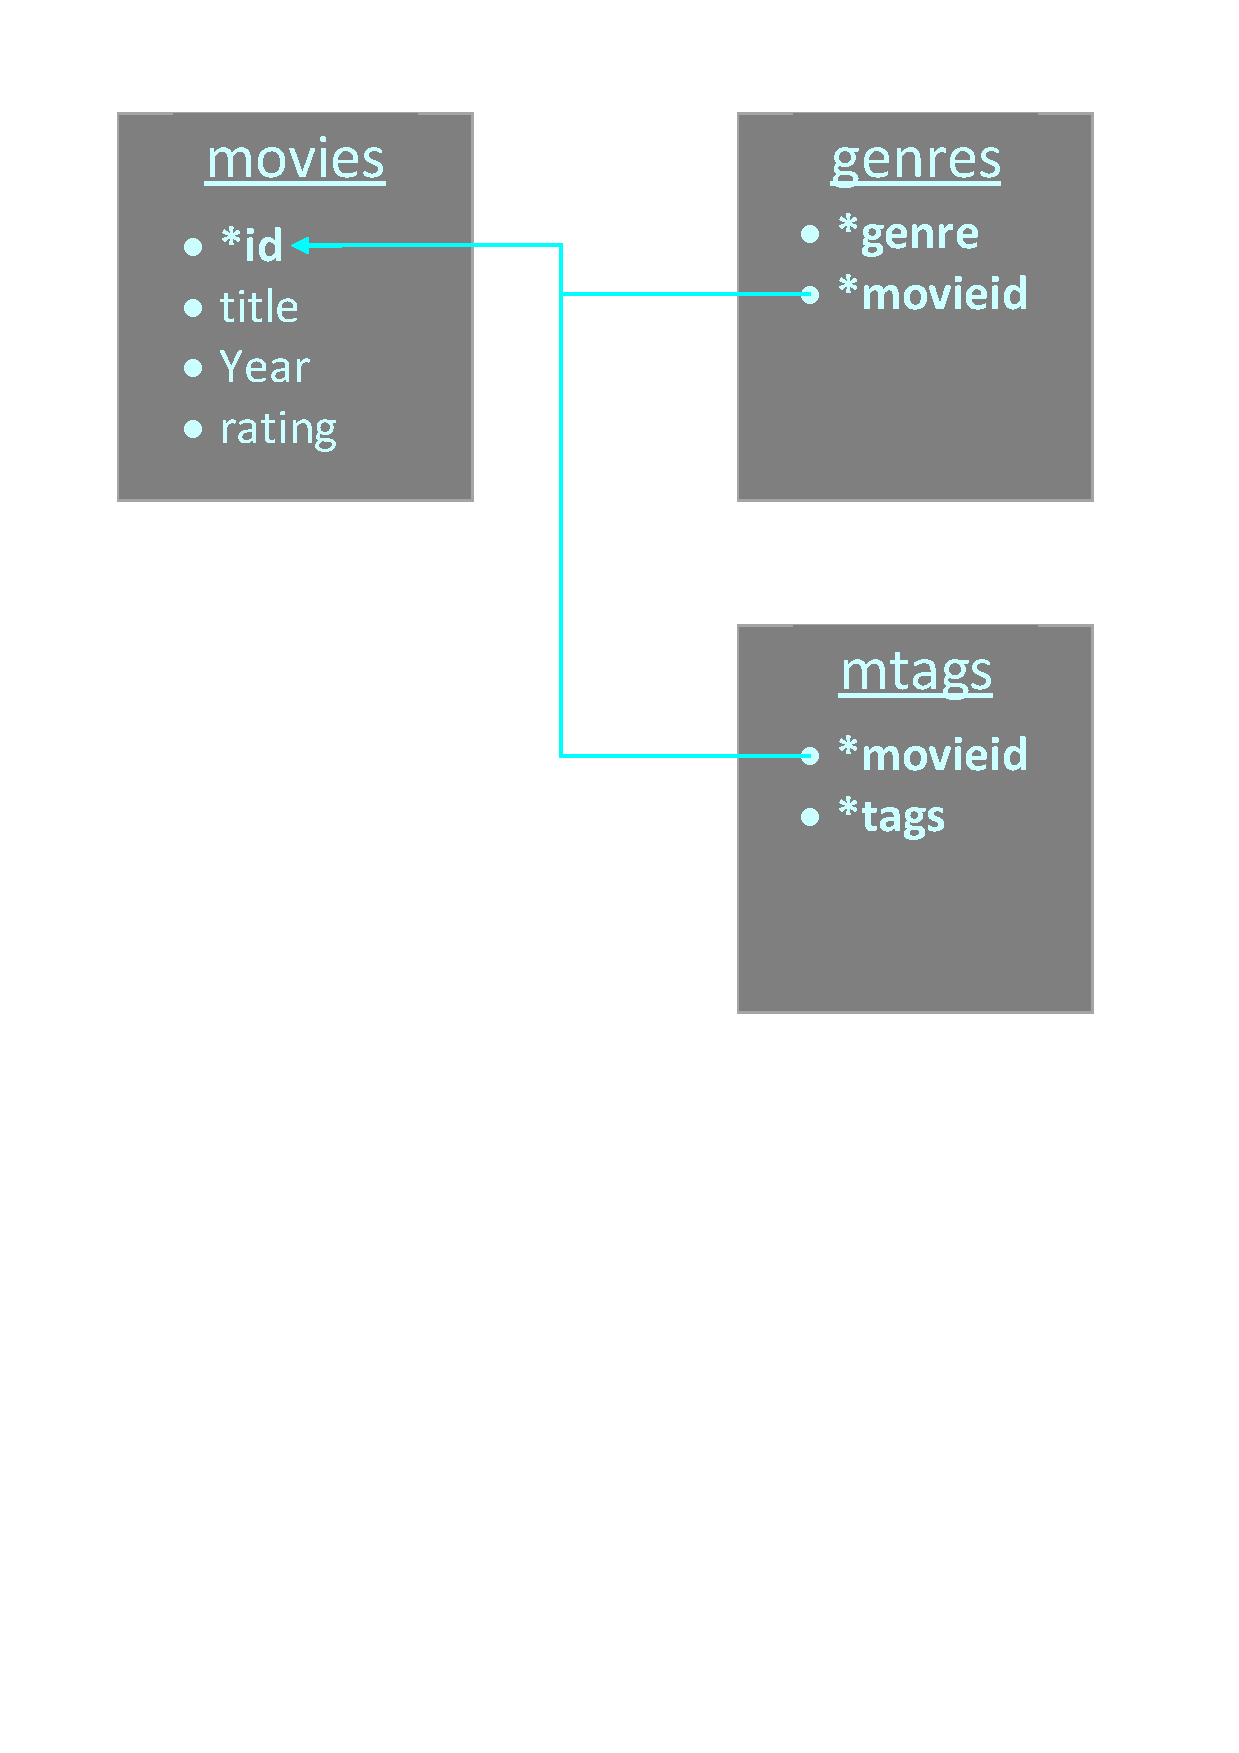
\includegraphics[width=13cm, trim = 0pt 11cm 0pt 1cm, clip]{ds.pdf}
	\caption{Database schema \label{fig:dataschema}}
\end{figure} 

%-----------------------------------------------------------------------------
%								Aðferð
%-----------------------------------------------------------------------------
\section{Aðferð}\label{nidurstodur}
\subsection{Hönnun}
Það var ákveðið að hafa GUI (Graphical user interface) og markmiðið var að hafa það sem einfaldast og notendavænast. Því hefur aðalgluggi forritisins (sbr.~Mynd \ref{fig:cdbf}) 2 dálka, eina leitarstiku og 5 hnappa.

Notast var við Qt4 Designer \cite{qt4} til að hanna GUI, það var valið með það í huga að það er auðvelt í notkun og við yrðum mun fljótari að hanna GUI á þann hátt.

\subsection{Virkni leita}
Á tveimur mismunandi stigum í forritinu er haft samband við gagnagrunninn. Annars vegar þegar leitað er að myndum sem notandanum líkar við, og hins vegar þegar leitað er að tillögum að myndum sem notandanum gæti líkað við.
\\
Finna myndir sem notanda líkar við, sbr.~Query \ref{lst:Search} í Appendix \ref{app:sql}:
\begin{itemize}
	\item Finna allar myndir/myndir frá ári þar sem hluti titilsins/ársins inniheldur leitarstrenginn
\end{itemize}
Finna tillögur að myndum sem notanda gæti líkað við:
\begin{itemize}
	\item Finna genres, sbr.~Query \ref{lst:genre} í Appendix \ref{app:sql}
	\begin{itemize}
		\item Finna genres kvikmynda/r sem notanda líkar við
	\end{itemize}
	\item Finna tög, sbr.~Query \ref{lst:tag} í Appendix \ref{app:sql}
	\begin{itemize}
		\item Finna tög sem eiga við myndir sem notanda líkar við
	\end{itemize}
	\item Finna tillögur að myndum, sbr.~Query \ref{lst:simmovies} í Appendix \ref{app:sql}
	\begin{itemize}
		\item Finna hvert og eitt tilvik af mynd sem tilheyrir einu af þeim genres eða hefur sama tag og einhver af myndunum sem notandanum líkar við, auk þess sem rating þarf að vera hærra en meðal-rating þeirra mynda sem notandanum líkar við, mínus hálfur.
		\item Raða myndum eftir því hversu oft þær koma fyrir
		\item Þær 10 myndir sem koma oftast fyrir er síðan raðað eftir rating
	\end{itemize}
\end{itemize}
\textbf{ATH: Töflur í gagnagrunni verða að heita þeim nöfnum sem sjást á Mynd \ref{fig:dataschema} annars virka leitarquery-in ekki.}

\subsection{Virkni forrits}
Þegar gui\_test.py skráin er keyrð opnast aðalgluggi forritisins (Mynd \ref{fig:cdbf}). Til að tengjast gagnagrunni er hægt að ýta á Ctrl + E (slaufa + E á mac) eða smellt á "Database" og valið "Edit info...". Þá opnast sprettigluggi þar sem upplýsingar um gagnagrunn eru settar inn, sjá Mynd \ref{fig:dbf2}. Eftir að ýtt er á "Ok" í sprettiglugganum birtist annar sprettigluggi sem lætur notandann vita hvort tekist hafi að tengjast gagnagrunninum.

\begin{figure}[h!]
	\centering 
	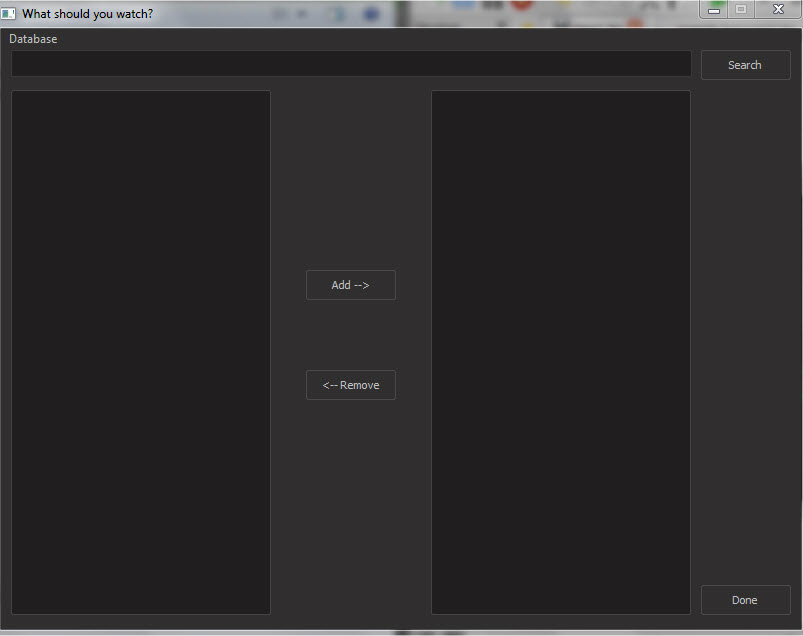
\includegraphics[width=13cm]{cdbf.png}
	\caption{Aðalgluggi forritsins \label{fig:cdbf}}
\end{figure}

\begin{figure}[h!]
	\centering 
	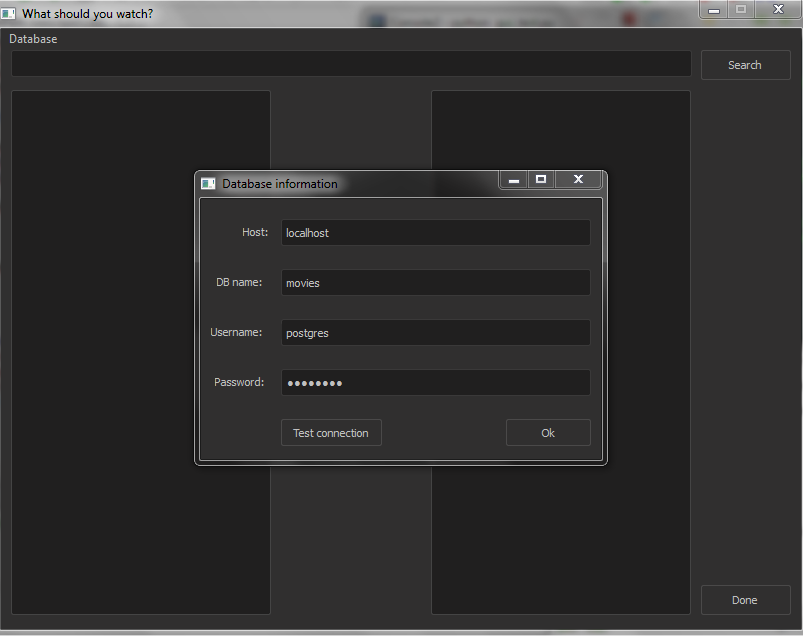
\includegraphics[width=13cm]{dbf2.png}
	\caption{Sprettiglugginn með upplýsingum útfylltum \label{fig:dbf2}}
\end{figure}

Þegar notandinn hefur tengst gagnagrunni getur hann leitað að mynd með því að skrifa nafn, eða hluta nafns, í leitarstikuna og ýtir svo á search (eða Return). Einnig er hægt að leita að útgáfuári, en þá er slegið ár inní leitarstikuna og fást þá allar myndir gefnar út á því ári.

Niðurstöður þeirrar leitarinnar birtast í vinstri dálknum. Ef notandanum líst á einhverja af myndunum sem koma upp við leitina getur hann bætt henni við á listann yfir myndir sem notandanum líkar við með því að ýta á á "add" hnappinn og þá færist valda myndin úr vinstri dálkinn yfir í hægri dálkinn, sjá Mynd \ref{fig:dbf6}. Ef notandinn vill taka myndir af listanum getur hann ýtt á "Remove" hnappinn og þá færist myndin úr hægri dálknum yfir í vinstri dálkinn aftur.

Þegar ýtt er á "done" hnappinn sprettur upp annar sprettigluggi sem kemur með tillögur að myndum sem notandanum gæti líkað við, sjá Mynd \ref{fig:dbf10}. Eftir það er hægt að prófa aðrar myndir með því að ýta á "yes" hnappinn, annars ýtir notandinn á "no" hnappinn og þá er forritinu lokað.

\begin{figure}
	\centering 
	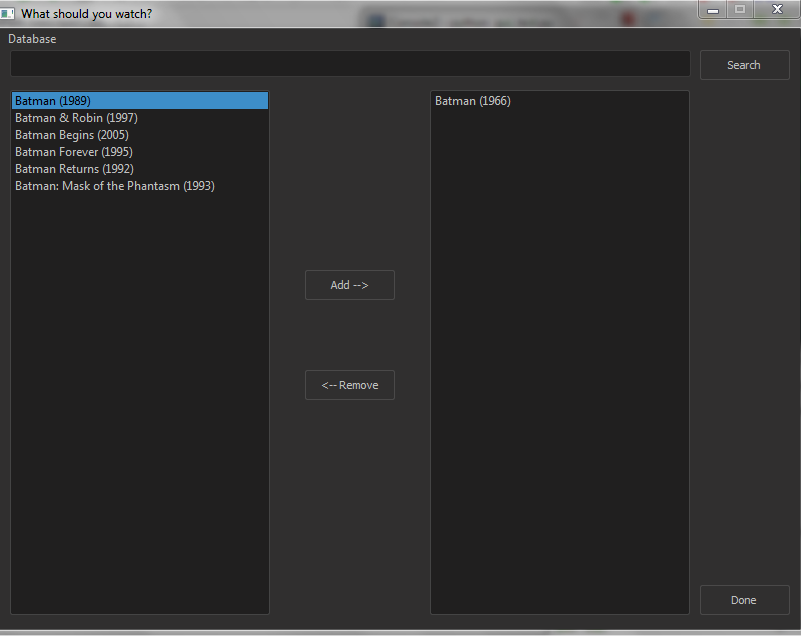
\includegraphics[width=13cm]{dbf6.png}
	\caption{Myndaleit skilar niðurstöðum í vinstri dálk\label{fig:dbf6}}
\end{figure}

\begin{figure}
	\centering 
	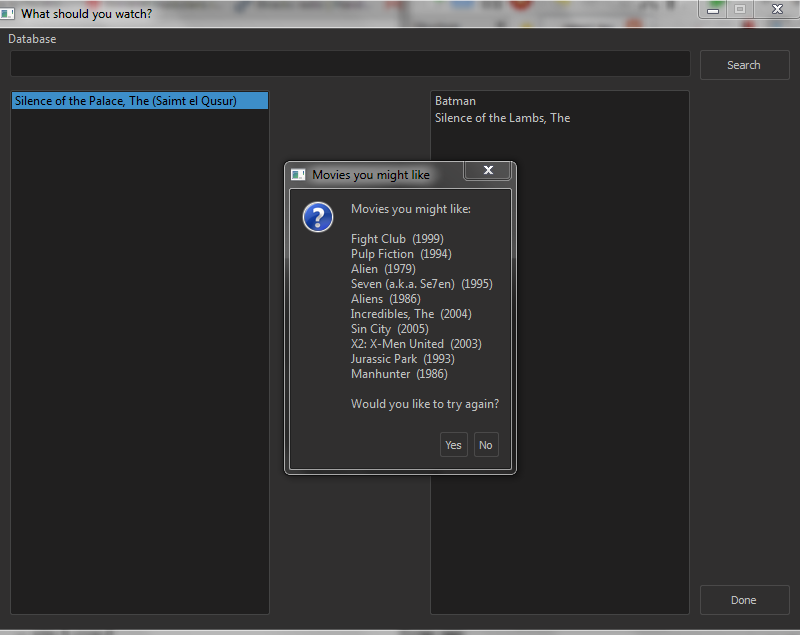
\includegraphics[width=13cm]{dbf10.png}
	\caption{Svipaðar myndir og þær sem settar voru í hægri dálkinn birtast í sprettiglugga\label{fig:dbf10}}
\end{figure}
\pagebreak
%-----------------------------------------------------------------------------
%								Niðurstöður
%-----------------------------------------------------------------------------
\section{Niðurstöður}
Að mati hópsins virkar forritið merkilega vel. Forritið skilar stöðugt svipuðum myndum og þeim sem notanda líkar við. Hins vegar á forritið erfiðara með að finna líkar myndir ef myndir sem notanda líkar við eru mjög ólíkar. Þetta verður að teljast eðlilegt þ.s.~forritið þarf þá að skoða mun fleiri gögn. Þrátt fyrir það eru tillögurnar samt sem áður góðar (hafa gott rating), en eru ekki endilega mjög líkar þeim myndum sem notanda líkar við.

Annað sem má nefna um niðurstöðurnar er að tögin eiga það til að gera niðurstöður frekar bjagaðar þegar um er að ræða vinsælar myndaseríur, þá sér í lagi teiknimyndir frá Pixar eða Disney. Þær valda því að meirihluti tillaga eru í þeim dúr.

Ef notandi setur inn 5 eða færri myndir sem honum líkar við tekur almennt minna en 3 sekúndur að finna tillögur að myndum. Eftir því sem myndirnar aukast tekur meiri tíma að finna tillögur en almennt tekur það ekki meira en 10 sekúndur.

Prófað var að setja inn allar myndir frá árinu 2000 og tók 1 mínútu og 22 sekúndur að finna tillögur að myndum. Líklega væri hægt að besta SQL query-in og láta python vinna minni vinnu við tilbúning þeirra, en ákveðið var að hafa kóðann eins og hann er vegna tíma og læsileika á það hvað er að gerast.
\\
Nokkur dæmi um notkun forritisins:
\begin{itemize}
	\item Myndir sem notanda líkar við:
	\begin{itemize}
		\item \textit{Batman}, \textit{Batman Begins}, \textit{Batman Forever}
	\end{itemize}
	\item Tillögur að myndum sem notanda gæti líkað við:
	\begin{itemize}
		\item \textit{Star Wars: Episode V - The Empire Strikes Back}  (1980), \textit{Lord of the Rings: The Fellowship of the Ring, The}  (2001), \textit{Pulp Fiction}  (1994), \textit{Snatch}  (2000), \textit{Incredibles, The}  (2004), \textit{X2: X-Men United}  (2003), \textit{Spider-Man}  (2002), \textit{Spider-Man 2}  (2004), \textit{X-Men}  (2000), \textit{Batman Returns}  (1992)
	\end{itemize}
	
	\item Myndir sem notanda líkar við:
	\begin{itemize}
		\item \textit{Iron Man}, \textit{Princess Mononoke}, \textit{A Bug's Life}, \textit{The Prestige}
	\end{itemize}
	\item Tillögur að myndum sem notanda gæti líkað við:
	\begin{itemize}
		\item \textit{Spirited Away (Sen to Chihiro no kamikakushi)}  (2001), \textit{Lord of the Rings: The Fellowship of the Ring, The}  (2001), \textit{Lord of the Rings: The Return of the King, The}  (2003), \textit{Blade Runner}  (1982), \textit{Nausicaä of the Valley of the Winds (Kaze no tani no Naushika)}  (1984), \textit{Howl's Moving Castle (Hauru no ugoku shiro)}  (2004), \textit{Incredibles, The}  (2004), \textit{Toy Story}  (1995), \textit{Kiki's Delivery Service} (Majo no takkyûbin)  (1989), \textit{Finding Nemo}  (2003)
	\end{itemize}
	
	\item Myndir sem notanda líkar við:
	\begin{itemize}
		\item \textit{Lucky Number Slevin}, \textit{The Shawshank Redemption}, \textit{Back to the Future}, \textit{WALL-E}, \textit{The Sixth Sense}, \textit{Psycho}, \textit{Ocean's Eleven}, \textit{Teenage Mutant Ninja Turtles}
	\end{itemize}
	\item Tillögur að myndum sem notanda gæti líkað við:
	\begin{itemize}
		\item \textit{Star Wars: Episode IV - A New Hope (a.k.a. Star Wars)}  (1977), \textit{Silence of the Lambs, The}  (1991), \textit{Princess Bride, The}  (1987), \textit{Blade Runner}  (1982), \textit{Eternal Sunshine of the Spotless Mind}  (2004), \textit{Seven (a.k.a. Se7en)}  (1995), \textit{Clockwork Orange, A}  (1971), \textit{Toy Story}  (1995), \textit{Sin City}  (2005), \textit{Jurassic Park}  (1993)
	\end{itemize}
\end{itemize}

\pagebreak
%-----------------------------------------------------------------------------
%								Appendix
%-----------------------------------------------------------------------------
\appendix
\section{SQL Queries} \label{app:sql}
\begin{lstlisting}[language = SQL, caption = Finna myndir sem notanda líkar út frá leitarstreng, label=lst:Search]
	select title, year, rating
	from movies
	where lower(title) like '%leitarstrengur%' or year like '%leitarstrengur%'
	order by title;
\end{lstlisting}

\begin{lstlisting}[language = SQL, caption = Finna genres út frá titlum og ári titla, label = lst:genre]
select distinct lower(g.genre)
from genres g, movies m
where m.id = g.movieid
and ( lower(m.title) = 'mynd1' and m.year = 'ar1'
or lower(m.title) = 'mynd2' and m.year = 'ar2'
or ...
)
order by lower(g.genre)
\end{lstlisting}

\begin{lstlisting}[language = SQL, caption = Finna tags út frá titlum og ári titla, label = lst:tag]
select distinct lower(mt.tag)
from genres g, movies m, mtags mt
where m.id = g.movieid and m.id = mt.movieid
and ( lower(m.title) = 'mynd1' and m.year = 'ar1'
or lower(m.title) = 'mynd2' and m.year = 'ar2'
or ...
)
order by lower(mt.tag)
\end{lstlisting}

\begin{lstlisting}[language = SQL, caption = Finna líkar myndir, label = lst:simmovies]
select m.title, m.year, m.rating
from movies m
where (m.title, m.year) in (
select m.title, m.year
from genres g, movies m, mtags mt
where m.id = g.movieid and m.id = mt.movieid
and m.rating >= (avg_input_rating - 0.5)
and ( lower(g.genre) = 'genre1' or lower(g.genre)='genre2'... )
and ( lower(mt.tag) = 'tag1' or lower(mt.tag) = 'tag2' ... )
and ( lower(m.title) != 'mynd1' and m.year != 'ar1'
and lower(m.title) != 'mynd2' and m.year != 'ar2'
...
)
group by m.title, m.year
order by count(m.title) desc
limit 10
)
order by m.rating desc;
\end{lstlisting}


\clearpage
\printbibliography

\end{document} % this tells the compiler that we are done

% These are variables for the editor Emacs
%%% Local Variables: 
%%% TeX-command-BibTeX: biber
%%% mode: latex
%%% TeX-master: t
%%% End:
